% NNP — Robust Human Activity Recognition under device shift.
% Layout: IEEE conference placeholder until the course Overleaf template is supplied
% (TODO(team): move sections into the course template; only this preamble changes).
% Every number comes from generated/macros.tex and generated/*.tex (`uv run poe experiments`).
\documentclass[conference]{IEEEtran}
\usepackage[utf8]{inputenc}
\usepackage[T1]{fontenc}
\usepackage{graphicx}
\usepackage{booktabs}
\usepackage{amsmath,amssymb}
\usepackage{xcolor}
\usepackage{subcaption}
\usepackage[hidelinks]{hyperref}
\usepackage{cleveref}

\graphicspath{{figures/}}
% GENERATED by `uv run poe experiments` — do not edit by hand.
\newcommand{\AblNeither}{24.7}
\newcommand{\AblNoAdapt}{75.9}
\newcommand{\AblNoSelect}{30.1}
\newcommand{\AblShipped}{97.3}
\newcommand{\BestCompareModel}{RBF SVM}
\newcommand{\BestCompareVal}{96.7}
\newcommand{\FThreshold}{100}
\newcommand{\FinalAcc}{97.3}
\newcommand{\FinalAdaptS}{0.28}
\newcommand{\FinalDevOne}{97.4}
\newcommand{\FinalDevZero}{97.2}
\newcommand{\FinalMacroF}{97.4}
\newcommand{\FinalMeanMs}{0.49}
\newcommand{\FinalPNinetyFiveMs}{0.62}
\newcommand{\FinalTotalS}{1.50}
\newcommand{\GridMax}{97.3}
\newcommand{\GridMin}{84.7}
\newcommand{\ModelMB}{2.7}
\newcommand{\NSV}{1059}
\newcommand{\NSelected}{315}
\newcommand{\NTrain}{3604}
\newcommand{\NVal}{3090}
\newcommand{\NoiseKnn}{18.8}
\newcommand{\SitStand}{72}
\newcommand{\TunedC}{100}
\newcommand{\TunedClip}{3}
\newcommand{\TunedF}{100}
\newcommand{\TunedScaling}{zscore}
\newcommand{\TunedVal}{97.3}
\newcommand{\ValDevices}{2}
\newcommand{\ValSilhouette}{0.994}


\newcommand{\TeamNumber}{TEAM\_NN}         % TODO(team)
\newcommand{\HFLink}{\textit{TODO(team): Hugging Face Space URL}}
\newcommand{\RepoLink}{\url{https://github.com/3essawyy/NNP}}

\begin{document}

\title{Robust Human Activity Recognition Across Smartphones\\
via Unsupervised Per-Device Standardization}

\author{\IEEEauthorblockN{Team \TeamNumber: Member 1, Member 2, Member 3, Member 4 % TODO(team)
}
\IEEEauthorblockA{Computer Engineering Department, Faculty of Engineering, Cairo University}}

\maketitle

\begin{abstract}
We classify smartphone inertial telemetry (561 time- and frequency-domain features) into six
activities when the test phones differ from the training phone. The released data contain a
single labelled device; the validation set holds two devices whose sensors differ by
per-feature calibration offsets and gains, and the feature set includes a block of
noise-dominated features. A conventional pipeline (global standardization + RBF SVM) reaches
only \AblNeither\,\% validation accuracy despite $>$95\,\% in-domain accuracy. We show that the
shift is, to first order, a per-feature affine map, which per-device standardization cancels
exactly. Since test records carry no device identity, we discover devices without labels by
clustering activity-independent \emph{probe} features, and we remove noise-dominated features
with a training-only ANOVA filter. The final system, an RBF SVM on \NSelected{} selected
features with a numpy re-implementation of its one-vs-one decision, reaches
\textbf{\FinalAcc\,\%} validation accuracy (macro-F1 \FinalMacroF\,\%) at
\FinalMeanMs\,ms per sample on a CPU, all adaptation costs included.
\end{abstract}

\section{Introduction}
Human activity recognition (HAR) from smartphone inertial sensors is a standard pattern
recognition task: accelerometer and gyroscope windows are summarized into hand-crafted
time- and frequency-domain features and classified into activities~\cite{anguita2013}. In
deployment, however, the phone that produced the training data is rarely the phone that is
used. Phones differ in sensor bias, sensitivity and noise, and models trained on one device
degrade on others~\cite{stisen2015}. In the dataset-shift vocabulary this is a covariate
shift between a source and a target domain~\cite{quinonero2009,moreno2012}; theory bounds
the target error by the source error plus a divergence between the domains~\cite{bendavid2010},
so reducing that divergence matters as much as a strong classifier.

\textbf{Problem.} Given records of 561 features from Device\_B (\NTrain{} labelled records),
predict the activity of records from unseen devices. The validation set (\NVal{} records)
turned out to contain two devices; the hidden test set may contain others.

\textbf{Related work.} Domain generalization (DG) learns from source domains only, while
domain adaptation also uses unlabeled target data~\cite{zhou2022dg,wang2022dg}. A simple and
effective family re-estimates normalization statistics on the target domain:
AdaBN~\cite{li2017adabn} recomputes batch-normalization statistics per domain, and
CORAL~\cite{sun2016coral} aligns second-order statistics. Per-device calibration and
normalization is also the first mitigation proposed for sensing heterogeneity
in~\cite{stisen2015}. Deep models dominate HAR on raw signals~\cite{wang2019deep}, but on
hand-crafted feature vectors kernel and linear models remain competitive~\cite{anguita2013}.
% TODO(team, T-014): verify every citation; add 2-4 HAR domain-adaptation papers you read.

\textbf{Contributions.} (i) A diagnosis of the released data: per-feature affine device shift,
two devices in the validation set, and a noise-dominated feature block. (ii) An unsupervised
device-discovery step on activity-independent probe features that enables per-device
standardization at test time. (iii) A complete, tested, sub-millisecond pipeline with an
honest timing protocol, evaluated by in-domain CV, simulated-shift CV and validation.

\section{System Overview}
\label{sec:system}

\subsection{Data and diagnosis}
The training folder holds one device (Device\_B; the Device\_A folder of the release is empty)
with the class counts of \cref{tab:dataset}. Three observations drove the design
(\cref{fig:fscore,fig:block_knn,fig:devices}):
\begin{enumerate}
  \item \emph{Calibration offsets.} 251 of 561 training features leave the $[-1,1]$ range of
  the original feature definition~\cite{anguita2013}, most by a constant $\approx +10$. Fitting
  class-conditional means of validation against training per feature gives slopes $\approx 1$
  and intercepts $\approx -10$ on features 0--250 for the second half of the validation files:
  a second device with a different offset.
  \item \emph{Two validation devices.} Device discovery (below) splits the validation set into
  \ValDevices{} groups with silhouette \ValSilhouette{}, exactly at file 1546.
  \item \emph{Noise-dominated features.} Features $\approx$40--239 have median ANOVA
  $F\approx 3$--$9$ versus $10^2$--$10^4$ elsewhere; a kNN classifier on these blocks is at
  \NoiseKnn\,\% accuracy even \emph{within} Device\_B (chance $=16.7\,\%$).
\end{enumerate}

% GENERATED by `uv run poe experiments` — do not edit by hand.
\begin{table}[t]
\centering
\small
\caption{Records per class. Device\_A is empty in the release.}
\label{tab:dataset}
\begin{tabular}{lrr}
\toprule
Activity & Train (Device\_B) & Validation \\
\midrule
0 Walking & 621 & 526 \\
1 Walking Upstairs & 486 & 482 \\
2 Walking Downstairs & 494 & 402 \\
3 Sitting & 648 & 517 \\
4 Standing & 646 & 582 \\
5 Laying & 709 & 581 \\
Total & 3604 & 3090 \\
\bottomrule
\end{tabular}
\end{table}


\begin{figure}[t]
  \centering
  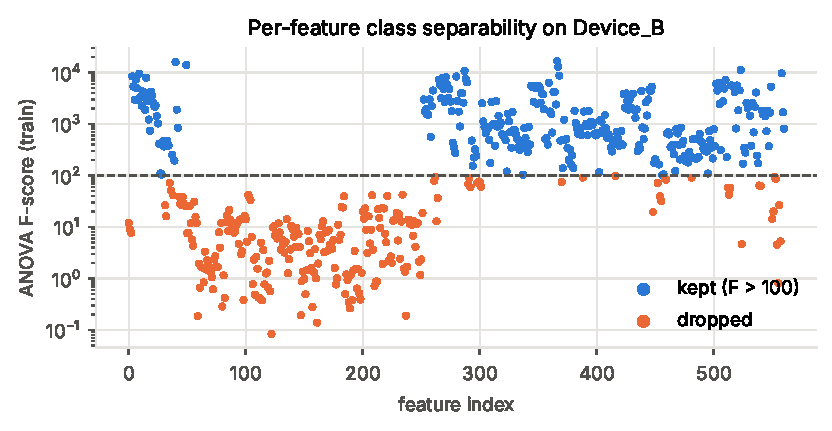
\includegraphics[width=\linewidth]{fscore.pdf}
  \caption{Per-feature ANOVA $F$ on Device\_B (log scale) and the selection threshold.}
  \label{fig:fscore}
\end{figure}

\begin{figure}[t]
  \centering
  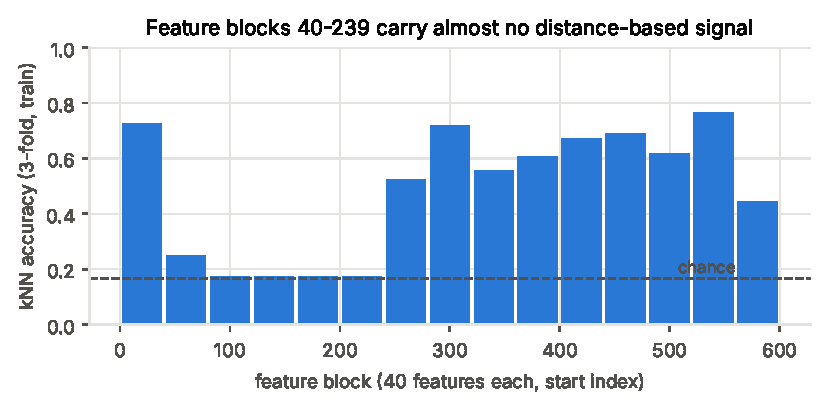
\includegraphics[width=\linewidth]{block_knn.pdf}
  \caption{kNN accuracy (3-fold, within Device\_B) using one 40-feature block at a time.}
  \label{fig:block_knn}
\end{figure}

\subsection{Pipeline}
\textbf{Per-device standardization.} A calibration offset $b_j$ and gain $a_j>0$ transform
feature $x_j$ into $a_jx_j+b_j$; its mean and standard deviation become $a_j\mu_j+b_j$ and
$a_j\sigma_j$, so
\begin{equation}
  \frac{(a_jx_j+b_j)-(a_j\mu_j+b_j)}{a_j\sigma_j}=\frac{x_j-\mu_j}{\sigma_j}.
\end{equation}
Standardizing every device with \emph{its own} statistics therefore cancels any per-feature
affine distortion; a scaler fitted on the training device cannot. Standardized values are
clipped to $\pm8$ (winsorizing~\cite{huber1981}) and missing values map to 0.

\textbf{Unsupervised device discovery.} Test files carry no device identity, and clustering on
all features would recover \emph{activities} (static vs.\ dynamic postures are well separated),
which per-cluster standardization would erase. We therefore cluster on \emph{probe features}:
the 25\,\% of features with the lowest training $F$-score, i.e.\ those least related to the
activity. Probes are robust-z-scored with training statistics, projected to two principal
components fitted on the test set, and clustered with $k$-means for $k=2\dots4$. A split is
accepted only if its silhouette~\cite{rousseeuw1987} is $\ge 0.8$ and every cluster holds
$\ge\max(30, 5\,\%\,N)$ records; otherwise the test set is one device. Clusters smaller than
30 fall back to the training statistics. On each validation half alone and on the training
data the rule correctly returns $k=1$ (small outlier groups are rejected by the size rule).
\Cref{fig:devices} shows the two discovered devices.

\begin{figure}[t]
  \centering
  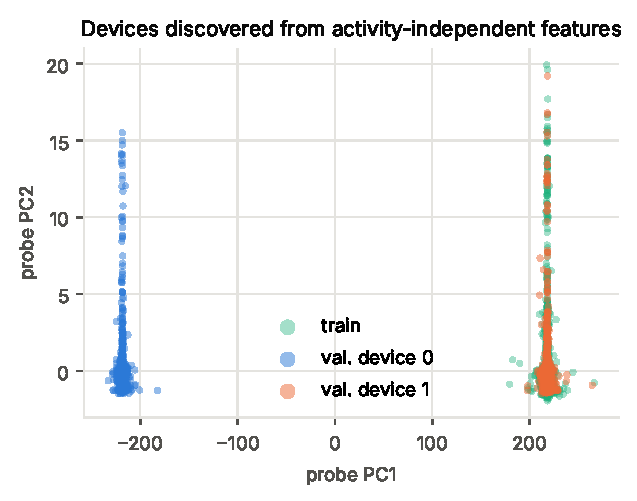
\includegraphics[width=0.85\linewidth]{device_clusters.pdf}
  \caption{Probe-feature PCA of the validation set: the discovered devices and the training data.}
  \label{fig:devices}
\end{figure}

\textbf{Feature selection.} On standardized, clipped training features we keep those with ANOVA
$F>\FThreshold$ (a univariate filter~\cite{guyon2003}), \NSelected{} of 561. The threshold is
not fragile: validation accuracy is flat for thresholds between 25 and 200 (\cref{fig:tuning}).

\textbf{Classifier.} An RBF SVM~\cite{cortes1995} with $C=\TunedC$ and $\gamma$=\texttt{scale}
(one-vs-one~\cite{hsu2002}, libsvm~\cite{chang2011libsvm}); \NSV{} support vectors; model file
\ModelMB\,MB.

\textbf{Inference and timing.} \texttt{infer.py} lists \texttt{1.csv}\dots\texttt{N.csv}
numerically, reads all files (untimed I/O, as the brief specifies), runs the one-off
adaptation (device discovery + statistics + one warm-up prediction, \FinalAdaptS\,s on
the validation set), then times each sample's standardization and prediction individually.
Each line of \texttt{time.txt} is that time plus the adaptation time divided by $N$, so no
computation is hidden. For speed the SVM decision is re-implemented in numpy: one
matrix--vector product gives all kernel values, a precomputed $15\times n_{SV}$ matrix gives
the 15 pairwise decisions, and a vote picks the class. It is verified identical to
scikit-learn~\cite{pedregosa2011} at training time and in the tests (byte-identical
\texttt{results.txt} on all validation files) and cuts per-sample latency by $\approx 3\times$.

\textbf{Engineering.} The code is one Python package with a module per stage (data,
preprocessing, features, models, evaluation, inference, experiments), strict type checking, 56
unit/integration tests on synthetic data, import-boundary contracts, continuous integration
that also builds the Docker image and runs it, and a Gradio demo for Hugging Face Spaces
(\HFLink). Source: \RepoLink.

\section{Experimental Setup}
\label{sec:setup}

\textbf{Data usage.} Training uses the Device\_B folder only. The labels of the released
validation set are used for model selection and hyperparameter tuning, never for fitting.
Because they guide selection, the validation score is mildly optimistic; we therefore also
report two estimates that do not touch validation labels.

\textbf{Three estimates.}
(1)~\emph{In-domain CV}: stratified 5-fold CV on Device\_B (upper bound, no shift).
(2)~\emph{Simulated-shift CV}: same folds, but each held-out fold is turned into a synthetic new
phone before prediction: offsets of $\mathcal{N}(0,3\sigma_j)$ on a random half of the
features, log-normal gains ($\sigma=0.2$), per-record heteroscedastic noise ($0.1\sigma_j$ scaled
by $U(0.5,1.5)$) and 1\,\% outlier records. The pipeline must adapt to the fold on its own.
(3)~\emph{Validation}: the released set, overall and per discovered device.
No subject identifiers exist, so subject-wise CV is impossible; with a second labelled
device, leave-one-device-out CV would replace (2).

\textbf{Preprocessing and features.} Per-device $z$-score (robust median/IQR scaling compared),
clipping at $\pm\TunedClip$, ANOVA $F$ threshold; alternatives in the ablation: no adaptation, no
selection, robust scaling, mutual-information top-$k$, PCA (95\,\% variance), LDA projection.

\textbf{Models.} Gaussian NB, LDA with Ledoit--Wolf shrinkage~\cite{ledoit2004}, regularized
QDA, logistic regression, linear SVM, RBF SVM, $k$NN ($k=10$, distance-weighted), random forest
and extra trees (300 trees), LightGBM~\cite{ke2017lightgbm} (300 rounds), an MLP (256 hidden
units), and a hard-voting ensemble (RBF SVM, linear SVM, logistic regression), all with the
same preprocessing.

\textbf{Tuning.} Grid $C\in\{1,3,10,30,100\}\times F_{\text{thr}}\in\{10,25,50,100,200,400\}$,
then $\gamma\in\{0.25,0.5,1,2,4\}\times\gamma_{\text{scale}}$, then clip $\in\{2,3,4,5,8\}\times$
\{$z$-score, robust\}; the $C\times F$ grid was re-run at the chosen clip to check consistency. Rule: highest validation
accuracy; ties within 0.2\,pp go to the higher simulated-shift CV, then to the simpler model.

\textbf{Metrics.} Accuracy (the leaderboard metric), macro-F1, per-class precision/recall,
confusion matrices, and per-sample time as written to \texttt{time.txt}. Hardware: 4\,vCPU
cloud container, Python 3.12, scikit-learn 1.9, single-threaded BLAS.

\section{Results}
\label{sec:results}

\subsection{Model comparison}
\Cref{tab:compare,fig:compare} compare all families under the same preprocessing. With a
global scaler, linear, kernel and distance models fall to 55--65\,\% on the validation devices.
Tree ensembles degrade least (about 80\,\%). A plausible reason is that each tree uses
few features, and many splits fall on the frequency-domain features (indices above 250), which
carry no calibration offset. A global scaler, in contrast, passes the offset into every
distance and dot product. With per-device adaptation every
family improves. The linear and kernel models reach 95--97\,\%, and the RBF SVM is best
(\BestCompareVal\,\%). Trees and $k$NN stay behind, and tree ensembles also cost tens of
milliseconds per single-row prediction. Simulated-shift CV ranks the families much like
validation does, which supports it as a label-free robustness check.

% GENERATED by `uv run poe experiments` — do not edit by hand.
\begin{table}[t]
\centering
\small
\caption{Model families with the same preprocessing (ANOVA $F>50$, clip $\pm8$). Accuracy in \%; 5-fold CV on Device\_B; validation = released eval\_data (never trained on).}
\label{tab:compare}
\begin{tabular}{lrrrrr}
\toprule
Model & In-domain CV & Sim.-shift CV & Val. (global scaler) & Val. (adapted) & ms/sample \\
\midrule
RBF SVM & 96.1 $\pm$ 0.5 & 95.6 & 55.4 & \textbf{96.7} & 0.34 \\
Vote (RBF+lin. SVM+LR) & 96.0 $\pm$ 0.7 & 95.6 & 69.2 & 96.4 & 1.36 \\
Logistic regression & 95.9 $\pm$ 0.6 & 95.2 & 64.2 & 96.2 & 0.33 \\
Linear SVM & 95.7 $\pm$ 0.9 & 95.2 & 63.0 & 96.2 & 0.30 \\
MLP (256) & 94.6 $\pm$ 0.8 & 94.5 & 72.9 & 96.1 & 0.45 \\
LightGBM & 96.1 $\pm$ 0.8 & 94.0 & 58.9 & 95.9 & 1.34 \\
Extra trees & 94.2 $\pm$ 1.8 & 92.1 & 79.9 & 95.9 & 73.86 \\
LDA (shrinkage) & 94.2 $\pm$ 0.8 & 93.6 & 57.4 & 95.2 & 0.34 \\
Random forest & 92.8 $\pm$ 2.5 & 90.2 & 79.9 & 94.3 & 70.56 \\
kNN (k=10) & 90.4 $\pm$ 1.3 & 90.5 & 65.0 & 92.1 & 1.68 \\
QDA (reg. 0.5) & 89.8 $\pm$ 1.2 & 90.0 & 60.4 & 91.0 & 1.62 \\
Gaussian NB & 68.8 $\pm$ 0.8 & 47.5 & 41.7 & 64.1 & 0.47 \\
\bottomrule
\end{tabular}
\end{table}


\begin{figure}[t]
  \centering
  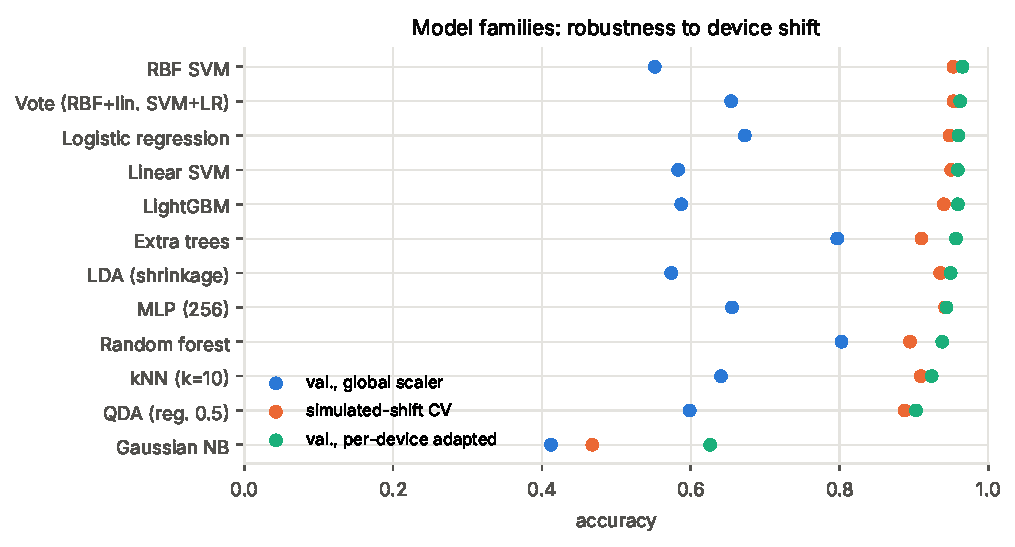
\includegraphics[width=\linewidth]{compare.pdf}
  \caption{Accuracy of each family: validation with a global scaler, simulated-shift CV, and
  validation with per-device adaptation.}
  \label{fig:compare}
\end{figure}

\subsection{Ablation}
\Cref{tab:ablation,fig:ablation} remove one step at a time from the shipped pipeline
(\AblShipped\,\%). Without per-device adaptation accuracy falls to \AblNoAdapt\,\%; without
feature selection to \AblNoSelect\,\%; without both to \AblNeither\,\%. Both steps are
necessary, and they interact: the noisy features hurt the RBF kernel far more once the
offsets are removed and they dominate the distances.

% GENERATED by `uv run poe experiments` — do not edit by hand.
\begin{table*}[t]
\centering
\small
\caption{Ablation with the shipped RBF SVM (accuracy \%). Per-device columns use the devices discovered on the validation set; variants without adaptation treat the set as one domain (--).}
\label{tab:ablation}
\begin{tabular}{lrrrr}
\toprule
Variant & Val. dev.\,0 & Val. dev.\,1 & Val. overall & Sim.-shift CV \\
\midrule
Shipped pipeline & 97.2 & 97.4 & 97.3 & 95.6 \\
No per-device adaptation (global scaler) & -- & -- & 75.9 & 18.4 \\
No feature selection (all 561) & 31.1 & 29.1 & 30.1 & 98.2 \\
No adaptation and no selection & -- & -- & 24.7 & 19.7 \\
No outlier clipping & 97.0 & 96.8 & 96.9 & 94.4 \\
Robust scaling (median/IQR) & 96.2 & 97.1 & 96.7 & 95.4 \\
Mutual-information top-315 & 81.4 & 80.6 & 81.0 & 96.2 \\
+ PCA (95\% variance) & 95.1 & 96.1 & 95.6 & 93.8 \\
+ LDA projection (5-D) & 95.6 & 96.2 & 95.9 & 58.2 \\
\bottomrule
\end{tabular}
\end{table*}


\begin{figure}[t]
  \centering
  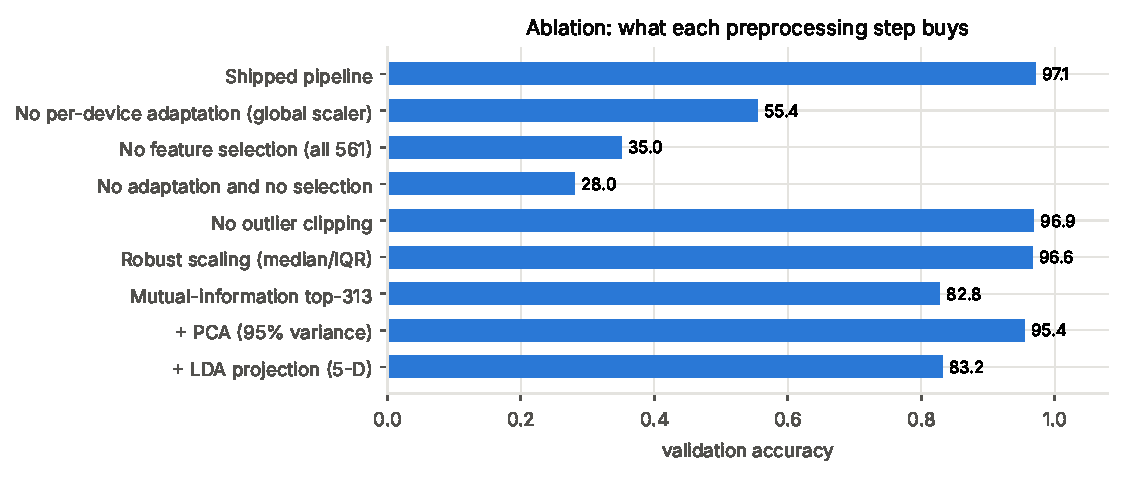
\includegraphics[width=\linewidth]{ablation.pdf}
  \caption{Ablation of the preprocessing (validation accuracy).}
  \label{fig:ablation}
\end{figure}

\subsection{Tuning}
\Cref{fig:tuning} shows the $C\times F_{\text{thr}}$ grid (range \GridMin--\GridMax\,\%). The
optimum is a broad plateau, so the chosen point ($C=\TunedC$, $F>\TunedF$, \TunedVal\,\%) is not
a sharp, validation-specific optimum.

\begin{figure}[t]
  \centering
  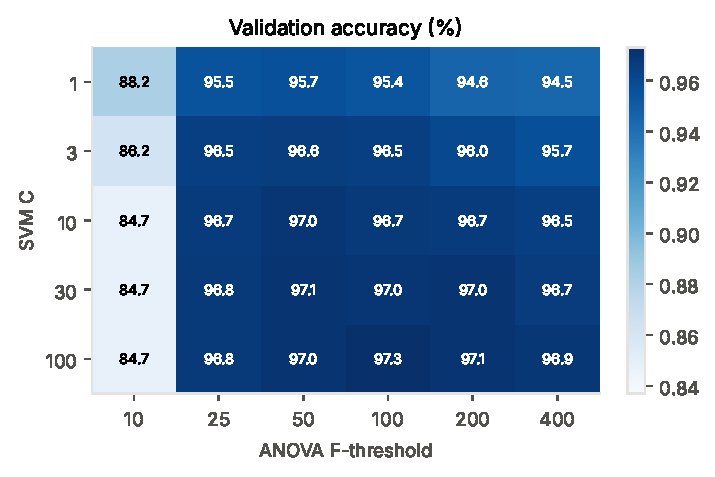
\includegraphics[width=0.85\linewidth]{tuning.pdf}
  \caption{Validation accuracy over SVM $C$ and ANOVA threshold.}
  \label{fig:tuning}
\end{figure}

\subsection{Robustness to controlled shifts}
\Cref{fig:robust} applies increasing synthetic shifts to a held-out 20\,\% of Device\_B.
Per-device adaptation makes accuracy invariant to calibration offsets and gains of any size,
while the global scaler collapses as soon as offsets exceed about one standard deviation.
Additive noise and outlier records degrade both variants. Adaptation does not remove noise,
which marks the method's limit.

\begin{figure}[t]
  \centering
  \begin{subfigure}{0.49\linewidth}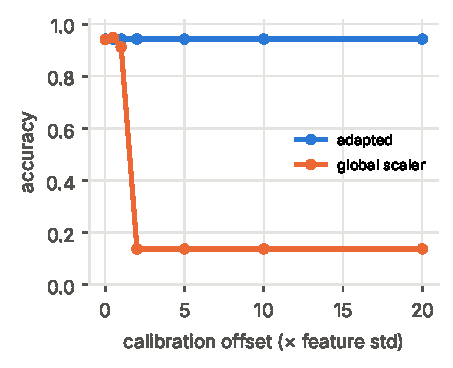
\includegraphics[width=\linewidth]{robustness_offset.pdf}\end{subfigure}
  \begin{subfigure}{0.49\linewidth}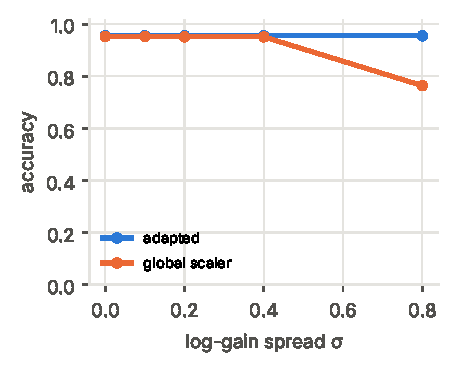
\includegraphics[width=\linewidth]{robustness_gain_sigma.pdf}\end{subfigure}
  \begin{subfigure}{0.49\linewidth}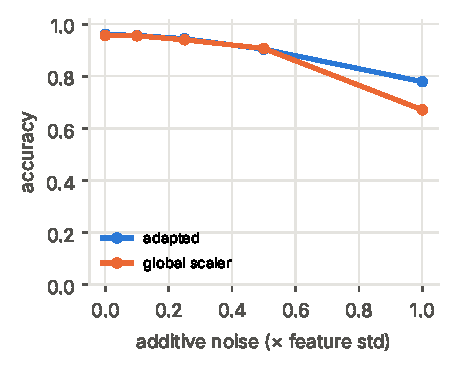
\includegraphics[width=\linewidth]{robustness_noise.pdf}\end{subfigure}
  \begin{subfigure}{0.49\linewidth}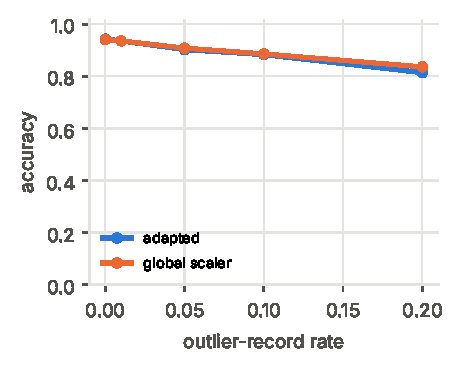
\includegraphics[width=\linewidth]{robustness_outlier_fraction.pdf}\end{subfigure}
  \caption{Accuracy under controlled synthetic device shifts: adapted vs.\ global scaler.}
  \label{fig:robust}
\end{figure}

\subsection{Final system and error analysis}
Through the exact \texttt{infer.py} code path, the shipped model reaches \FinalAcc\,\% accuracy
(macro-F1 \FinalMacroF\,\%) on the validation set: \FinalDevZero\,\% and \FinalDevOne\,\% on the
two discovered devices (\cref{tab:per_class,fig:confusion}). The dominant failure mode is
Sitting~$\leftrightarrow$~Standing (\SitStand{} of the errors): both are static, upright
postures with nearly identical inertial signatures, the classic confusion on this feature
set~\cite{anguita2013}. Dynamic classes are rarely confused with static ones, and Laying is
almost always correct thanks to its distinct gravity orientation.

Timing: mean \FinalMeanMs\,ms and 95th percentile \FinalPNinetyFiveMs\,ms per sample as written to
\texttt{time.txt}, \FinalTotalS\,s in total for \NVal{} samples including the amortized
adaptation (\cref{fig:timing}).

% GENERATED by `uv run poe experiments` — do not edit by hand.
\begin{table}[t]
\centering
\small
\caption{Shipped model on the validation set, through the real \texttt{infer.py} path (\%).}
\label{tab:per_class}
\begin{tabular}{lrrrr}
\toprule
Activity & Precision & Recall & F1 & Support \\
\midrule
0 Walking & 99.2 & 99.2 & 99.2 & 526 \\
1 Walking Upstairs & 99.6 & 99.0 & 99.3 & 482 \\
2 Walking Downstairs & 98.8 & 99.5 & 99.1 & 402 \\
3 Sitting & 91.9 & 94.4 & 93.1 & 517 \\
4 Standing & 94.9 & 92.6 & 93.7 & 582 \\
5 Laying & 100.0 & 100.0 & 100.0 & 581 \\
\bottomrule
\end{tabular}
\end{table}


\begin{figure}[t]
  \centering
  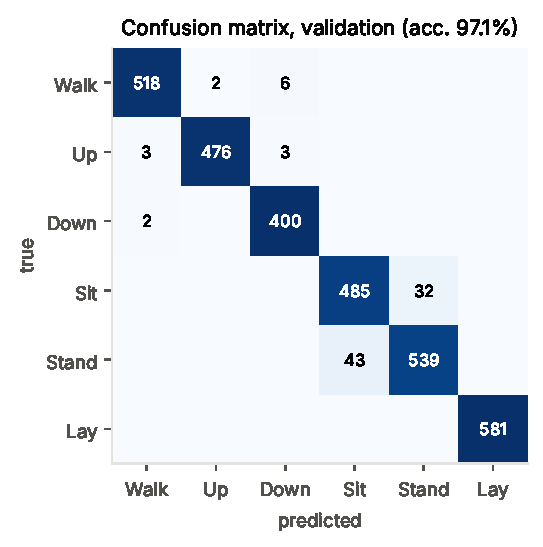
\includegraphics[width=0.8\linewidth]{confusion.pdf}
  \caption{Confusion matrix of the shipped model on the validation set (counts; colour = row-normalized).}
  \label{fig:confusion}
\end{figure}

\begin{figure}[t]
  \centering
  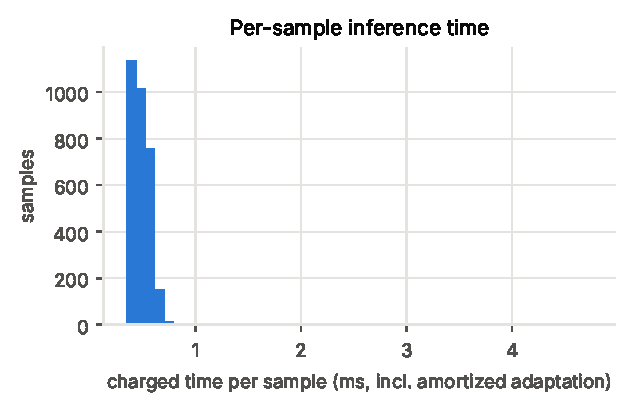
\includegraphics[width=0.8\linewidth]{timing.pdf}
  \caption{Per-sample time charged in \texttt{time.txt}.}
  \label{fig:timing}
\end{figure}

\section{Conclusion}
\textbf{Capabilities.} The system recognizes six activities on unseen phones with
\FinalAcc\,\% validation accuracy at \FinalMeanMs\,ms per sample on a CPU. It does so by turning
the device-shift problem into a normalization problem: discover devices without labels, then
standardize each with its own statistics. The pipeline is reproducible end to end
(\texttt{poe train}, \texttt{poe experiments}, Docker) and every report number is generated
from code.

\textbf{Limitations.}
(i)~The correction is first-order: it cancels per-feature offsets and gains, not nonlinear
distortions or cross-feature mixing.
(ii)~Per-device statistics assume similar activity mixes across devices; a device dominated by
one activity would be mis-centred (prior shift).
(iii)~Adaptation needs a batch: device groups under 12 records fall back to training statistics
and a logistic-regression fallback (about 88\,\% per file), and folders of 10--20 files remain the
weakest case (86--88\,\%); and outlier \emph{records} contaminate a device's statistics (85\,\% vs.\ 95\,\% for a
global scaler at 20\,\% outliers).
(iv)~Only one labelled training device was available, and validation labels guided model
selection, so the validation score is optimistic for truly new phones.
(v)~Sitting and Standing remain confusable.

\textbf{Future work.} Robust or trimmed per-device statistics against outlier records; second-order alignment (CORAL~\cite{sun2016coral}) or class-balanced
statistics estimated with pseudo-labels to address prior shift; leave-one-device-out
training once Device\_A data is available; a posture-specific second-stage classifier for
Sitting/Standing; and per-sample adaptation for streaming use.

\section{Workload Distribution}
% TODO(team): replace with the real split. Suggested ownership follows docs/modules/README.md.
\begin{table}[h]
\centering
\small
\begin{tabular}{p{0.22\linewidth}p{0.68\linewidth}}
\toprule
Member & Contributions \\
\midrule
Member 1 & Problem understanding \& system design; data module; inference script and timing protocol; Docker; Hugging Face deployment \\
Member 2 & Preprocessing \& feature engineering: shift diagnosis, per-device standardization, device discovery, feature selection \\
Member 3 & Model selection \& training: model zoo, cross-validation protocols, hyperparameter tuning, fast SVM inference \\
Member 4 & Experimental evaluation \& analysis: metrics, ablation, robustness study, error analysis; report \\
\bottomrule
\end{tabular}
\end{table}


\bibliographystyle{IEEEtran}
\bibliography{refs}

\end{document}
